\chapter{The Gravwell REST API}

\section{Introduction}
Gravwell implements a REST API over HTTP. This API powers the Gravwell UI, but it can also be used to interface other systems with Gravwell. For instance, a Python script can run a Gravwell query by hitting a single API endpoint. This chapter discusses \emph{API Tokens}, which are special authentication tokens given to client applications for accessing the API, and demonstrates how to access perhaps the most userful REST endpoint: the direct search API.

\section{Tokens}

Gravwell users can generate tokens which allow an application to act as that user, but with limited privileges. Tokens are passed to the Gravwell webserver with HTTP requests as a method of authentication. Tokens are managed through the Tokens page (Figure \ref{fig:token-page}), accessible in the Main Menu under the ``Tools and Resources'' section.

\begin{figure}
	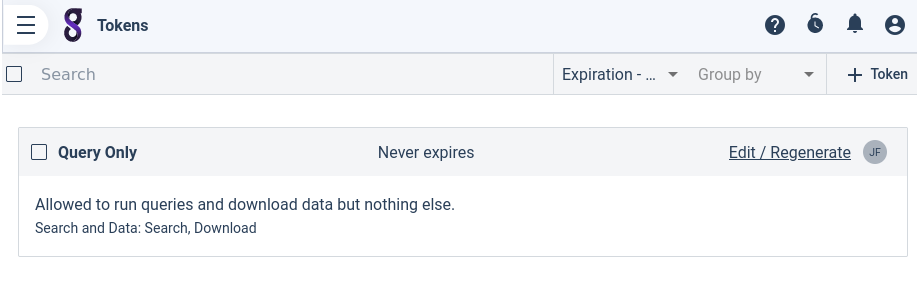
\includegraphics[width=0.8\linewidth]{images/token-page.png}
	\caption{The token management page.}
	\label{fig:token-page}
\end{figure}

New tokens are created by clicking the ``+ Token'' button in the upper right. This brings up a page where the token's name and description may be specified and a list of permissions can be selected. Figure \ref{fig:new-token} demonstrates how fine-grained capabilities can be assigned; in this example, the token will be able to run searches, download the results, get a list of tags, and even ingest additional entries, but it will \emph{not} be able to mark searches for saving or view search history. By carefully selecting permissions, it is possible to restrict the potential for harm if an API token is leaked.

\begin{figure}
	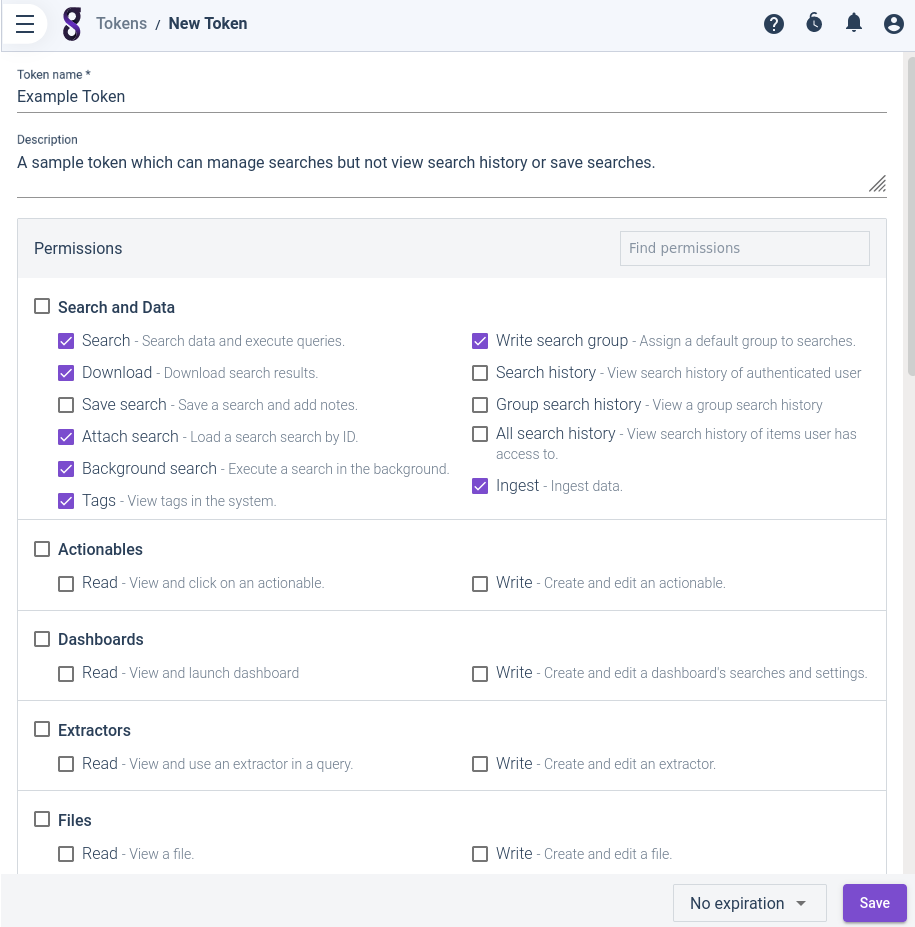
\includegraphics[width=0.8\linewidth]{images/new-token.png}
	\caption{Defining a new token.}
	\label{fig:new-token}
\end{figure}

Tokens can be set to expire after a period of time. By default, tokens last indefinitely, but the dropdown at the bottom of the new token page can be used to set a limited duration as seen in Figure \ref{fig:token-expiration}.

\begin{figure}
	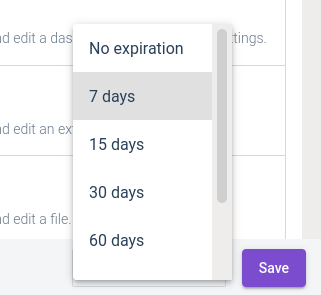
\includegraphics[width=0.4\linewidth]{images/token-expiration.png}
	\caption{Token expiration options.}
	\label{fig:token-expiration}
\end{figure}

Once permissions have been selected for the new token, clicking ``Save'' will bring up a dialog showing the secret key for the token (Figure \ref{fig:token-secret}. This key should be copied at this time; it cannot be retrieved again later.

\begin{figure}
	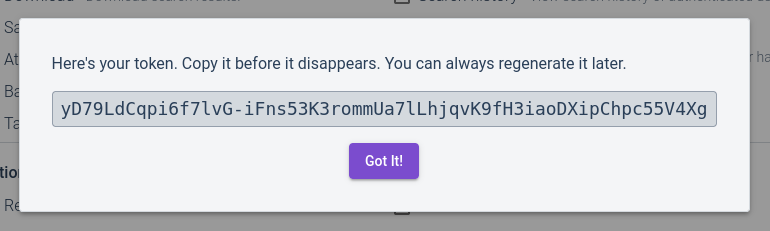
\includegraphics[width=0.7\linewidth]{images/token-secret.png}
	\caption{Token secret.}
	\label{fig:token-secret}
\end{figure}

If the secret is lost, the token can be \emph{regenerated}, creating a new secret key, but any applications using the old secret will stop working until updated.

\subsection{Token Permissions and Restrictions}

Token permissions are defined using specific allowances, in which the user selects exactly which functionality a given token is allowed to perform.  The Gravwell user interface provides some nice features to let you select groups of permissions that might be logically related, but in the end each token must declare exactly what APIs and systems it is allowed to access.  Most permissions are divided into read and write components.  This means a token might be configured so it can read resources but not write them, or a token can read the state of automation scripts but not create, update, or schedule them.

Permissions on tokens are an overlay on the user's existing permissions.  This means that if the current user cannot access an API or feature, then the token cannot either--tokens can only restrict access, they cannot grant access that a user does not currently have.

Note: The `Token write' permission can be particularly dangerous. If you grant a token the ability to write to the token API, it can create new tokens with any permission it wants.  Token permissions are not transitive, so a restricted token with access to the `Token Write' permission could create new tokens with no restrictions.

The token system only provides access to user-level APIs and cannot be used by admins to access admin-level APIs.  An admin can still create and use tokens, but they cannot access APIs that require admin permissions.  For example, an admin cannot use a token to create users or update a license.

\section{Accessing the Gravwell API}

There are many, many REST endpoints in the Gravwell API. A reasonably complete listing is available on the Gravwell documentation site.\footnote{\href{https://docs.gravwell.io/\#!api/api.md}{https://docs.gravwell.io/\#!api/api.md}} The easiest way to interact with the API is using the \code{curl} command. Authentication is done by including a token secret (as described above) into a header named ``Gravwell-Token''. For example, to fetch a list of tags in the system:

\begin{verbatim}
% curl -H 'Gravwell-Token: DQ-Tgpe56czTSZ_kzzDlFqqMKSkIR65hOoTmcdUK0J-7DMq3H2YmDK-0WQ' \
	http://gravwell.example.org/api/tags
["default","syslog","kernel","dmesg","windows","www","netflow","ipfix"]
\end{verbatim}

\section{Direct Search API}
The Gravwell Direct Query API is designed to provide atomic, REST-powered access to the Gravwell query system.  This API allows for simple integration with external tools and systems that do not normally know how to interact with Gravwell.  The API is designed to be as flexible as possible and support any tool that knows how to interact with an HTTP API.

The Direct Query API is authenticated and requires a valid Gravwell account with access to the Gravwell query system; a Gravwell token is the best way to access the API.

Issuing a query via the Direct Query API requires the same set of parameters as issuing a query via the Gravwell web GUI: a query string, a time range, and an optional output format.  The Direct Query API has some limitations on which output formats can be provided.  For example, the pointmap and heatmap renderers cannot output rendered maps via this API, nor can this API draw a chart and deliver it as an image.  This API is primarily used for retrieving raw results and delivering them to other systems for direct integration.

The Direct Query API is atomic: one request will execute an entire search and deliver the completed results.  Queries that cover large time ranges or require significant time to execute may require that HTTP clients adjust their respective client timeouts.

\subsection{Query Endpoints}

The Direct Query API consists of two REST endpoints which can parse a search and execute a search.  The parse API is useful for testing whether a query is valid and could execute while the search API will actually execute a search and deliver the results.  Both the query and parse APIs require the user and/or token to have the `Search` permission.

\subsubsection{Parse API}

The parse API is used to validate the syntax of a Gravwell query before attempting to execute it. The parse API is accessed via a POST request to \code{/api/parse}.  The parse API a query string delivered by header value, URL parameter, or a ParseSearchRequest\footnote{https://pkg.go.dev/github.com/gravwell/gravwell/v3/client/types\#ParseSearchRequest} JSON object.  A ParseSearchResponse\footnote{https://pkg.go.dev/github.com/gravwell/gravwell/v3/client/types\#ParseSearchResponse} object and a 200 code will be returned if the query is valid.

The following curl commands are all functionally equivalent:

\begin{verbatim}
curl -X POST \
   -H "Gravwell-Token: aFOa_YbO7Pe0MAqK08PSD-oTrEZxopc5JBf0hu0W5_Vo-FxWsjHp" \
   -H "query: tag=gravwell limit 10" \
   http://10.0.0.1/api/parse
\end{verbatim}

\begin{verbatim}
curl -X POST \
   -H "Gravwell-Token: aFOa_YbO7Pe0MAqK08PSD-oTrEZxopc5JBf0hu0W5_Vo-FxWsjHp" \
   http://10.0.0.1/api/parse?query=tag%3Dgravwell%20limit%2010
\end{verbatim}

\begin{verbatim}
curl -X POST -H -d '{"SearchString":"tag=gravwell limit 10"}' \
   "Gravwell-Token: aFOa_YbO7Pe0MAqK08PSD-oTrEZxopc5JBf0hu0W5_Vo-FxWsjHp" \
   http://10.0.0.1/api/parse
\end{verbatim}

An example response is shown below:

\begin{verbatim}[H]
{
  "Sequence": 0,
  "GoodQuery": false,
  "ParsedQuery": "tag=gravwell limit 10",
  "RawQuery": "tag=gravwell limit 10",
  "ModuleIndex": 0,
  "CollapsingIndex": 1,
  "RenderModule": "text",
  "TimeZoomDisabled": false,
  "Tags": [
    "gravwell"
  ],
  "ModuleHints": [
    {
      "Name": "limit",
      "ProducedEVs": null,
      "ConsumedEVs": null,
      "ResourcesNeeded": null,
      "Condensing": true
    },
    {
      "Name": "limitCollapser",
      "ProducedEVs": null,
      "ConsumedEVs": null,
      "ResourcesNeeded": null,
      "Condensing": true
    },
    {
      "Name": "sort",
      "ProducedEVs": null,
      "ConsumedEVs": null,
      "ResourcesNeeded": null,
      "Condensing": false
    }
  ]
}
\end{verbatim}

\subsubsection{Query API}

The query API actually runs a search and returns the results. It is accessed via a POST to \code{/api/search/direct}. The search API requires the parameters in Table \ref{table:query-parameters} be delivered by header values, URL parameters, or a JSON object.

\begin{table}[H]
\begin{tabular}{llc}
\hline
\textbf{Parameter} & \textbf{Description} & \textbf{Optional} \\
query     & A complete Gravwell query string & \\
format    & Query output format & \\
preview   & Boolean indicating that the query should execute as a preview query & yes \\
start     & RFC3339 start timestamp for the query & yes \\
end       & RFC3339 end timestamp for the query & yes \\
duration  & Go-encoded duration & yes \\
\end{tabular}
\caption{Query Request Parameters}
\label{table:query-parameters}
\end{table}

Note that while the `start', `end', and `duration' parameters are optional at last one complete set must be provided, either `start' and `end' or `duration'.

The results of the query are returned in the body of the response. Each query renderer will support a different set of output formats. If the specified output format is not supported a 400 BadRequest response will be returned.

The following are all valid invocations; the first example shows a sample result as well:

\begin{verbatim}
% curl -X POST \
   -H "Gravwell-Token: aFOa_YbO7Pe0MAqK08PSD-oTrEZxopc5JBf0hu0W5_Vo-FxWsjHp" \
   -H "query: tag=gravwell stats count" \
   -H "duration: 1h" \
   -H "format: text" \
   http://10.0.0.1/api/search/direct
count 14599
\end{verbatim}

\begin{verbatim}
% curl -X POST \
   -H "Gravwell-Token: aFOa_YbO7Pe0MAqK08PSD-oTrEZxopc5JBf0hu0W5_Vo-FxWsjHp" \
   'http://10.0.0.1/api/search/direct?query=tag%3Dgravwell%20stats%20count&format=text&duration=1h'
\end{verbatim}

\begin{verbatim}
% curl -X POST \
   -H "Gravwell-Token: aFOa_YbO7Pe0MAqK08PSD-oTrEZxopc5JBf0hu0W5_Vo-FxWsjHp" \
   -d '{"SearchString":"tag=gravwell stats count","SearchStart":"2022-03-01T12:00:00Z",
"SearchEnd":"2022-03-01T13:00:00Z","Format":"text"}' \
   http://10.0.0.1/api/search/direct
\end{verbatim}

This example mixes some parameters in a JSON object, some as headers, and some as URL parameters:

\begin{verbatim}
% curl -X POST \
   -H "Gravwell-Token: aFOa_YbO7Pe0MAqK08PSD-oTrEZxopc5JBf0hu0W5_Vo-FxWsjHp" \
   -d '{"SearchString":"tag=gravwell limit 10"}'
   -H 'duration: 1h' \
   http://10.0.0.1/api/search/direct?format=text
\end{verbatim}

This example fetches the results in CSV format:

\begin{verbatim}
% curl -X POST \
   -H "Gravwell-Token: aFOa_YbO7Pe0MAqK08PSD-oTrEZxopc5JBf0hu0W5_Vo-FxWsjHp" \
   -H "query: tag=gravwell syslog Appname | stats count by Appname | table Appname count" \
   -H "duration: 1h" \
   -H "format: csv" \
   http://10.0.0.1/api/search/direct
\end{verbatim}

This example fetches the results as raw PCAP and stores the output in \code{/tmp/port80.pcap}:

\begin{verbatim}
% curl -X POST \
   -H "Gravwell-Token: aFOa_YbO7Pe0MAqK08PSD-oTrEZxopc5JBf0hu0W5_Vo-FxWsjHp" \
   -H "query: tag=packets packet tcp.Port==80 ipv4.IP==192.168.1.1 | pcap" \
   -H "duration: 1h" \
   -H "format: pcap" \
   --output /tmp/port80.pcap \
   http://10.0.0.1/api/search/direct
\end{verbatim}
